\documentclass{article}
\usepackage{graphicx}
\usepackage{float}
\usepackage{amssymb}
\usepackage{amsmath}
\usepackage{mathrsfs}
\usepackage{bm}
\usepackage{mathtools}
\usepackage{fullpage}
\usepackage{wrapfig}
\usepackage{hyperref}

\newcommand{\norm}[1]{\left\lVert#1\right\rVert}

\begin{document}

\title{Wasserstein Riemannian Frameworks}
\author{Octav Dragoi}

\maketitle

\begin{abstract}
    The point of this short writeup is to describe how to construct
    Riemannian-like objects, such as geodesics, tangent spaces, 
    exponential and log maps, etc, over the space of point clouds
    endowed with the Wasserstein metric.
\end{abstract}

\section{Introduction}

\subsection{Definitions}
Let $X$ be a Riemannian manifold, in our case we can take $X=\mathbb{R}^d$
for some $d$. In literature, the space $\mathscr{P}_2(X)$ is
defined as the space of all Borel measures over $X$ with finite second moments
(we need this condition to ensure the existence of the Wasserstein distance).

There are two important ways in which these measures relate, through 
transport plans and transport maps. We shall define each one in turn. 
Let $\mu \in \mathscr{P}_2(X), \nu \in \mathscr{P}_2(Y)$.
\begin{itemize}
    \item A \textbf{transport map} is simply a function $T:X\rightarrow Y$
    for which $\nu = T_\#\mu$.  The measure $T_\#\mu\in \mathscr{P}_2(Y)$ is 
    called the \textit{pushforward of $\mu$ through $T$} and is defined as:
    \[T_\#\mu(E) = \mu(T^{-1}(E)),\ \forall E\subset Y\text{ Borel} \]

    Intuitively, this is a point to point mapping from $X$ to $Y$ that
    preserves the $\mu$ measure on the image set.

    \item A \textbf{transport plan} is a measure 
    $\bm\gamma \in \mathscr{P}_2(X\times Y)$,
    for which the marginals agree with $\mu$ and $\nu$, specifically:
    \[\bm\gamma(A\times Y) =\mu(A), \bm\gamma (X\times B) = \nu(B)\]

    Denote by $\textsc{Adm}(\mu, \nu)$ the set of all transport maps 
    between $\mu$ and $\nu$.

    Intuitively, this is a pairing that describes how much weight 
    is transported from each point to possibly more points in the image set.
    This is a generalization of transport maps, since weight from one point 
    can (and usually does) flow into multiple points. Formally,
    each transport map $T$ can be expressed as a transport plan:
    \[\nu = T_\#(\mu)\implies \bm\gamma \coloneqq (Id\times T)_\#\mu\in\textsc{Adm}(X\times Y) \]
\end{itemize}

\subsection{Discussion on point clouds}

It is important to see how we can apply this theory to our point cloud embeddings.
The theory is defined on \textit{continuous} probability distributions across
$X$, whereas point clouds are inherently discrete. Therefore, we want to restrict
ourselves to looking at \textbf{measures with finite support}.

Under this constraint, transport maps become quite restrictive. Basically,
they only move points to other points, keeping the probability distribution
fixed between them, at most merging two points together. We need to see 
whether, for our purposes, this kind of restriction is workable.

Transport plans, where one point can be mapped to a multitude of other ones,
grant us much wider movement space, at the cost of more complex parametrization.
We shall see exactly how this is reflected mathematically, in the next 
section.

\section{The weak Riemannian structure of $(\mathscr{P}_2(X), W_2)$}

The Wasserstein distance $W_2$ between $\mu$ and $\nu$ is 
defined as:
\[W_2(\mu, \nu) = \sqrt{\inf_{\bm\gamma\in \textsc{Adm}(\mu, \nu)} \int d^2(x,y)d\bm\gamma(x,y)} \]

If $X$ is a Riemannian manifold, as it is in our case where $X=\mathbb{R}^d$,
then $(\mathscr{P}_2(X), W_2)$ is also a Riemannian manifold. In 
\cite{Ambrosio2013AUG}, the authors describe the topology of $(\mathscr{P}_2(X), W_2)$
and the construction of a Riemannian-like framework by mostly looking at
transport maps, not at transport plans.

As defined in \cite{Ambrosio2013AUG}, the set $\mathscr{P}_2(X)$ contains all 
distributions, but for our use case we would like to restrict this to 
probabilities with finite support, where each distribution is a sum of 
discrete weighted Dirac indicator distributions. Something like:
\[\mathscr{D}_2(X) = \left\{X = \sum_{i=1}^{n}\lambda_i\delta_{x_i} : 
n\in \mathbb{N}, \lambda_i\in\mathbb{R}, x_i\in X \right\} \]

Details have to be ironed out, but from the subsequent constructions it
looks likely that $(\mathscr{D}_2(X), W_2)$ also shares the same 
Riemannian-like structure.

\subsection{Geodesics and tangent spaces induced by transport maps}

If $X$ is a geodesic space, then for $t\mapsto \gamma_t$ a constant speed
geodesic between $x,y\in X$, then $t\mapsto \delta_{\gamma_t}$ is a 
constant speed geodesic over $\mathscr{P}_2(X)$. The natural way of 
taking geodesics therefore is by this so-called \textit{displacement 
interpolation}, i.e. taking intermediary points along the geodesic 
curve between two points. This is good; this process should therefore
generate new point clouds, rather than just shifting weight between
already defined points.

To illustrate the previous point, let us consider a simple example, with
two distributions $\mu = \delta_x, \nu = \delta_y$, for some $x, y\in X$. 
The geodesic $(\mu_t) \subset \mathscr{P}_2(X)$, for which $\mu_0 = \mu, 
\mu_1 = \nu$, is then defined accordingly as:
\[\mu_t = \delta_{tx + (1-t)y} \]

Notice that it is not $t\delta_x + (1-t)\delta_y$; this interpolation
process actually yields new points from $X$, rather than just 
redistributing weight among existing points.

Also notice that, if $\mu$ and $\nu$ have finite support, then also 
$\mu_t$ will have finite support (i.e. both of them are point clouds 
in $(\mathscr{D}_2(X), W_2)$).

In generaal, an optimal map $T$ naturally gives rise to ("induces") 
a constant speed geodesic $(\mu_t)\subset \mathscr{P}_2(X)$
on $\mathscr{P}_2(X) = \mathscr{P}_2(\mathbb{R}^d)$:
\[\mu_t = ((1-t)Id + tT)_\#\mu_0 \]
for which, if $\mu_0, \mu_1\in \mathscr{D}_2$, then $(\mu_t)\subset\mathscr{D}_2$.

Based on this, one can define the "instantaneous velocity" $v_t$ 
along this curve:
\[ v_t\coloneqq (T-Id)((1-t)Id + tT)^{-1}\]
which satisfies the continuity equation:
\begin{equation}
    \label{eq:continuity}
    \frac{d}{dt}\mu_t + \nabla \cdot (v_t\mu_t) = 0
\end{equation}

It is natural to think that integrating the instantaneous velocity along 
the geodesic curve should give us an indication of the curve's length.
The \textbf{Benamou-Brenier} formula recovers the Wasserstein distance
under this "dynamic" formulation:
\[W_2(\mu^0, \mu^1) = \inf\left\{ \int_0^1\norm{v_t}_{\mu_t}dt\right\} \]
where the infimum ranges over all solutions $(\mu_t, v_t)$ of (\ref{eq:continuity})
which link $\mu_0$ and $\mu_1$. If these vectors $v_t$ are induced by an
optimal transport plan, then the infimum is attained there and the 
integral is indeed equal to the Wasserstein distance.

These vectors $v_t$ of minimal size describe the movement of curves 
around $\mu_t$, so we want to define the tangent space as the collection 
of all such vectors, in a rigorous manner. Turns out, we can do this 
in two equivalent ways, actually.
\begin{itemize}
    \item The fact that these vectors act only on smooth functions suggests
    we should consider all gradients of such functions, or, more rigorously:
    \begin{equation}
        \label{eq:tgvect1}
        \overline{\left\{\nabla \phi : \phi\in C^\infty_c(X) \right\}}^{L_2(\mu)}
    \end{equation}
    \item Wanting to consider only $v_t$ of minimal norm, from the continuity
    eqauation \ref{eq:continuity}, one can check that this is equivalent to 
    having $v_t$ in the set:
    \begin{equation}
        \label{eq:tgvect2}
        \left\{v\in L^2(\mu_t) : \int\langle v,w\rangle d\mu_t = 0,\ \forall w \in L^2(\mu_t)\ s.t.\ \nabla\cdot(w\mu_t) = 0\right\}
    \end{equation}
\end{itemize}

The expressions from (\ref{eq:tgvect1}) and (\ref{eq:tgvect2}) are the same!
Therefore, the tangent space is defined as:
\begin{align*}
    \label{eq:tgvect}
    \text{Tan}_\mu(\mathscr{P}_2(X))&\coloneqq \overline{\left\{\nabla \phi : \phi\in C^\infty_c(X) \right\}}^{L_2(\mu)} \\
    &= \left\{v\in L^2(\mu) : \int\langle v,w\rangle d\mu = 0,\ \forall w \in L^2(\mu)\ s.t.\ \nabla\cdot(w\mu) = 0\right\}
\end{align*}

\subsection{Generalization to transport plans}

\cite{Ambrosio2013AUG} also discuss an alternative definition to the tangent space.
Define: 
\[\text{Geod}_\mu \coloneqq \{\text{geodesics starting from} \mu\}/\approx \]
where $(\mu_t)\approx (\mu_t')$ if they coincide on a neighborhood around $\mu$.

The natural distance on this space is:
\[D((\mu_t), (\mu_t')) = \overline{\lim}_{t\downarrow 0} \frac{W_2(\mu_t, \mu_t')}{t}\]

Then define the \textit{geometric tangent space} $\textbf{Tan}_\mu(\mathscr{P}_2(\mathbb{R}^d))$
as the completion of $\text{Geod}_\mu$ with respect to $D$.

This description is purposefully vague; since we will likely only use the solutions
over transport maps, where computations are usually more tractable and most of 
the literature is concentrated anyway, this part does not necessarily concern 
us directly.

\subsection{Discussion}

The bolded, larger "space of directions" $\textbf{Tan}_\mu(\mathscr{P}_2(\mathbb{R}^d))$ 
is larger than the "space of gradients" $\text{Tan}_\mu(\mathscr{P}_2(\mathbb{R}^d))$.
For example, if $\mu = \delta_x$ for some $x\in \mathbb{R}^d$, then:
\[\text{Tan}_\mu(\mathscr{P}_2(\mathbb{R}^d)) \sim \mathbb{R}^d \]  
however:
\[(\textbf{Tan}_\mu(\mathscr{P}_2(\mathbb{R}^d)), D) \sim (\mathscr{P}_2(\mathbb{R}^d), W_2)  \]

This intuitively happens because when displacing a point with a tangent map,
it inevitably gets sent to another point, so the set of all directions is isomorphic to
$\mathbb{R}^d$. However, when displacing a point with a transport plan, we can
essentially recover any distribution over our space, i.e. the set of all 
directions is $\mathscr{P}_2(\mathbb{R}^d)$.

We don't even need to go here, though, and this is the reason why that section 
only throws a furtive glance at general transportation plans. When solving Wasserstein 
transport plans for point cloud embeddings with an equal number of vertices, we actually 
retrieve transport maps. That's because the $W_2$ distance is convex in linear 
combinations of transport plans, since the $L^2$ distance is also convex
and therefore the minimum will be attained in points on the border of 
the transportation polytope.

\section{Principal Geodesic Analysis - Computing in Practice}
The main problem with the aforementioned concepts of tangent spaces and exponential maps
is that most of the computations
are intractable for an infinite-dimensional space like $\mathscr{P}_2(X)$. In the paper
\cite{seguy2015principal}, the authors describe a series of approximations for 
tangent vectors and interpolations in the $W_2$ space, together with algorithmic
implementations for the case of $\mathscr{D}_2(X)$. The paper's goal is 
to eventually arrive at a PCA-like analysis within Wasserstein spaces, but 
we shall use it rather for its computational framework.

For computations of Wasserstein barycenters, the authors of \cite{seguy2015principal}
use other implementations of other algorithms, such as \cite{benamou2014iterative} or 
\cite{cuturi2013fast}. Most of the geometric constructions that they devise then,
are actually used to compute the so-called "principal geodesics" and conduct 
some form of principal component analysis.

\subsection{Theory}
Let $\{\mu_i : 1\leq i\leq n, n\in \mathbb{N}\}\subset \mathscr{D}_2(X)$
be a finite set of probability measures with finite support, and let $\bar{\mu}$
be its average within the Wasserstein space. A geodesic through $\bar\mu$ is
parametrized by a vector $v\in L^2(\bar\mu)$ on a neighborhood around $\bar\mu$
as:
\[g_t(v)\coloneqq (id + tv)_\#\bar\mu \]
In \cite{ambgigli2006}, Lemma 7.2.1. shows that \textit{all} geodesics
through $\bar\mu$ are parametrized in such a way, so this does not restrict
the generality in any way. However, making sure that this is a geodesic is 
no trivial matter, and proves to be computationally too intensive. Therefore,
the authors adopt a relaxed definition of a geodesic, built upon \textit{two}
vector fields arount $\bar\mu$.

{

\begin{wrapfigure}{r}{0.4\textwidth}
    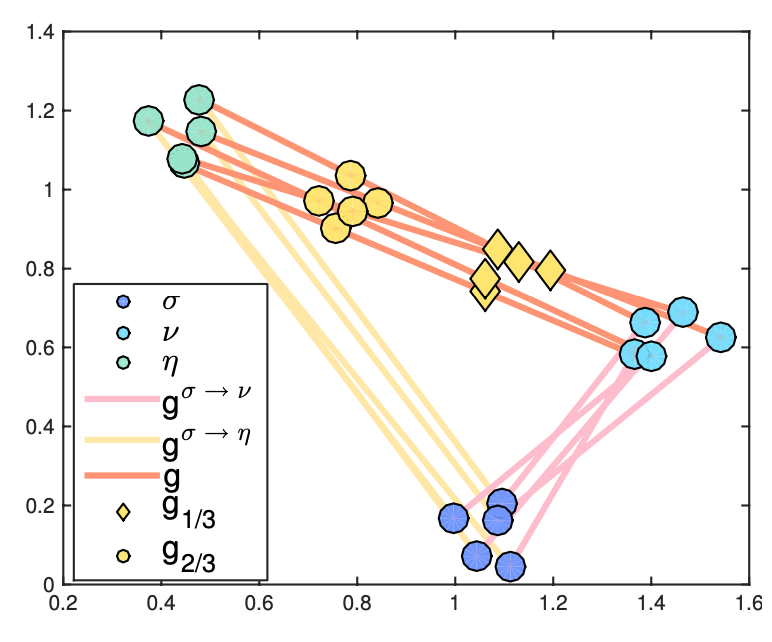
\includegraphics[trim={0 1cm 0 1.5cm},width=\linewidth]{images/generalized_geodesics.png}
    \caption{Generalized geodesic interpolation between two measures $\nu$
    and $\eta$ using a base measure $\sigma$, all within $\mathscr{P}_2(X)$}
    \label{fig:generalized_geodesics}
\end{wrapfigure}

Let $\sigma,\nu,\eta\in\mathscr{P}_2(X)$ and take optimal mappings $T^{(\sigma, \nu)}$
and $T^{(\sigma,\eta)}$ from $\sigma\rightarrow\nu$ and $\sigma\rightarrow\eta$, respectively.
A \textit{generalized geodesic} between $\nu$ and $\eta$ with base $\sigma$ is 
defined as:
\[g_t = \left((1-t)T^{(\sigma, \nu)} + tT^{(\sigma, \eta)}\right)\#\sigma,\ t\in[0,1] \]

In our case, for $\sigma = \bar\mu$ and $v_1, v_2$ two vector fields such that
$id-v_1, id+v_2$ are optimal mappings, the generalized geodesic can be written as:
\[g_t(v_1, v_2)\coloneqq \left(id - v_1 + t(v_1+v_2)\right)\#\bar\mu,\ t\in[0,1]  \] 

In Figure \ref{fig:generalized_geodesics} the authors of \cite{seguy2015principal}
illustrate how these generalized geodesics look like, for $t=\frac{1}{3}$ and 
$t = \frac{2}{3}$. The linear behavior of this kind of interpolation makes it 
cheaper to compute than the purely theoretical method.

}

\subsection{Computations in practice}

The Wasserstein mean $\bar\mu$ of the input measures $(\mu_i)$ is given,
and we denote $\bar\mu = \sum_{k=1}^pb_k\delta_{y_k}$, where $\sum b_i=1$
and $Y=[y_1,\dots, y_p]\in \mathbb{R}^(d\times p)$ is the matrix containing
the support of $\bar\mu$. In \cite{seguy2015principal}, they treat this $\bar\mu$
as given, and they compute it using some other barycentric algorithm.

For each of the $p$ points in $\bar\mu$, they consider \textit{two} velocity 
vectors. These vectors are represented by $V_1=[v_1^1,\dots,v_p^1]$ and  
$V_2=[v_1^2,\dots,v_p^2]$ in $\mathbb{R}^{d\times p}$. Under the assumption
that these velocity fields yield optimal mappings, the generalized geodesic
is defined as:
\[g_t(V_1, V_2) = \sum_{k=1^p}b_k\delta_{z^t_k} \]
where the locations $Z_t$ are computed as:
\[ Z_t = [z_1^t,\dots,z_p^t] \coloneqq Y-V_1 + t(V_1+V_2)\]


\subsection{Discussion}

In summary, this problem takes a set of point clouds as input, and constructs 
a geodesic emanating from their Frechet mean that minimizes the distance 
to them. This geodesic encapsulates the set's "information", in a similar 
manner to how a principal component does, in a vector space.

At this point, only the specific setup of the algorithm to construct these
geodesics has been summarized here. To me it seems that this algorithm has
a good potential to be useful, if we are interested in computing these tangent 
vectors $V_1, V_2$ and the principal geodesics. That's a big \textbf{if}!

\section{Gradient Flows}

This problem is an \textit{initial value problem}: given an initial point 
$\mu\in \mathscr{P}_2(M)$ and a smooth function $F:\mathscr{P}_2(M)\rightarrow
\mathbb{R}$, we want to find a \textit{gradient flow} $(\mu_t)$ such that:
\begin{equation*}
\begin{cases}
    \mu_t' = -\nabla F(\mu_t) \\
    \mu_0 = \mu
\end{cases}       
\end{equation*}

These definitions, as well as the main ideas, are taken from \cite{craig2017gradient}.

Intuitively, this means that $(\mu_t)$ evolves in the direction of steepest 
descent of $F$. This formulation suits well the task of "improving" datapoints,
when starting from a given initial point and optimizing a given functional
over the Wasserstein space.

To compute the gradient flow of a specific function, we turn back to the 
continuity equation \ref{eq:continuity}:
\[\frac{d}{dt}\mu_t + \nabla \cdot (v_t\mu_t) = 0\]
which means that, in the Wasserstein space, all gradient flows are of the form:
\[v = -\nabla\frac{\partial F}{\partial \mu} \]

One common technique for approximating these gradient flows is to pursue 
\textit{particle approximation}. In general, these $\mu$ are continuous
variables, so one approximates them with a set of Dirac masses and then 
shifts the points in the directions of steepest descent.

We shall see two cases, when $v$ is nice, and when we need to approximate 
the function. For our case, we will most likely have to use the second
possibility.

\subsection{If $v$ is "nice"}

In a theoretical setting where the functional $F$ is well-behaved and the 
vector space is easy to compute, we can apply it to every Dirac mass.

We would like to find an approximate solution for the ODE:
\[\frac{d}{dt}\mu(x,t) + \nabla (v(x,t)\mu(x,t)) = 0 \]

We will do a displacement for every atom of $\mu$, with respect to the 
tangent vector space $v$, since $v$ is nicely determined. Formally, if:
\[\mu = \sum_{i=1}^n\delta_{x_i}m_i \] 
then each Dirac mass point will be shifted according to $v$:
\[\frac{d}{dt}x_i(t) = v(x_i(t), t),\ i\in\overline{1,n}\]
and obtain the gradient flow:
\[\mu(t) = \sum_{i=1}^n\delta_{x_i(t)}m_i \]

\subsection{JKO Scheme}

The paper \cite{zhang2018policy} has gone to the length of transposing the 
physics-inspired theory into a framework for policy optimization. They define 
a \textit{policy} as a distribution over an action space, which is essentially 
the same mathematical object as our point clouds. Then they use the JKO 
scheme to approximate their loss functions (for reinforcement learning, 
in their case) and perform particle optimization.

The inspiration for this scheme comes from the Euclidean case. On the 
space $\mathbb{R}^d$, the standard iterative step for the gradient 
descent method is formulated as:
\[x_{k+1} = x_k - \nabla F(x_{k+1})h \]
or, equivalently, solving the optimization problem:
\[x_{k+1} = \arg\min_{x\in \mathbb{R}^d} F(x)+ \frac{\norm{x - x_k}_2^2}{2h} \]

For the Wasserstein metric, in a similar fashion, 
\begin{equation}
    \label{eq:jkoupdate}
    \mu_{k+1} = \arg\min_{\mu\in\mathscr{P}_2(M)} F(\mu)+ \frac{W_2^2(\mu - \mu_k)}{2h}
\end{equation}

This seems intractable in the general case. However, there are multiple
types of approximating this process, if the functional $F$ has an appropriate 
form. These forms seem to be taken from physics theory, so maybe someone 
with more extensive physics knowledge can contribute here. In any case,
paper \cite{zhang2018policy} has a short yet comprehensive overview of this,
and they manage to restate their physics-unrelated problem into something 
that conforms to this form.

Specifically, $F$ needs to be of the form:
\[F(\mu)\coloneqq -\int U(\mathbf{x})\mu(\mathbf{x})dx + \int
\mu(\mathbf{x})\log(\mu(\mathbf{x}))d\mathbf{x} \]
where $U:\mathbb{R}^d\rightarrow \mathbb{R}^d$ is a function called the 
\textit{drift term.}

For this particular formulation, the process \ref{eq:jkoupdate} becomes 
equivalent to:
\[\mu_{k+1} = \arg\min_{\mu\in\mathscr{P}_2(M)} \mathbf{KL}(\mu\parallel p(\mathbf{x}))+ \frac{W_2^2(\mu - \mu_k)}{2h} \]
where $p(\mathbf{x})\coloneqq \frac{1}{Z}e^{U(\mathbf{x})}$ is the target 
distribution, and $\mathbf{KL}$ is the Kullback-Leibler divergence operator.

\subsection{Discussion}

Most likely, $v$ is not "nice", so we would have to apply the JKO scheme
and find a proper way of approximating the solutions. Hopefully one of 
the classic ways of approximating this function will work for us.

\bibliographystyle{ieeetr}
\bibliography{thesisbib}

\end{document}